\documentclass{jsarticle}
\usepackage[dvipdfmx]{graphicx}
\begin{document}

\title{身体動作と筋電量の関係性}
\author{平松亨隆}
\maketitle


\section{目的}
私を含めて人は、意識的に筋肉の伸縮を考えて体を動かすわけではない。例えば、上腕二頭筋を使うことを意識して腕を曲げる人はまずいないだろう。だから、私達はどのような筋活動で運動をしているのかということに興味を持った。そこで、今回は腕の屈伸運動に着目し、上腕二頭筋と上腕三頭筋がどのような筋活動をしてその運動をしているのか、を明らかにすることを本レポートの目的とした。しかしこのような反復運動の場合、運動の速度を上げるほどブレて制御がしにくくなるという問題があるため、速度に違いがある場合には筋活動も違う可能性がある。そのため、腕の屈伸運動は二つの速度で行うことにした。

\section{実験方法}
\subsection{運動計測}
下記の図\ref{fig:short}はもっとも腕を曲げた状態、図\ref{fig:long}は最も腕を伸ばした状態の図である。被験者にはこの2つの状態を繰り返す腕の曲げ伸ばし運動を、利き腕を使って、速度に関して何も指示を出していない場合と速く動かしてもらった場合の2パターンで計測をした。被験者には反射マーカーを肩、肘、手首につけてモーションキャプチャー(ライブラリ社:MoveTR)を使って1000 fpsで撮影した。また筋電センサ(ロジカルプロダクト社)を上腕二頭筋と上腕三頭筋に貼付し、筋電位をサンプリング周波数200 Hzで計測した。筋電センサとカメラの計測時間は同期をとり、20秒間計測していた。
\begin{figure}[h]
  \begin{minipage}{0.5\hsize}
    \begin{center}
      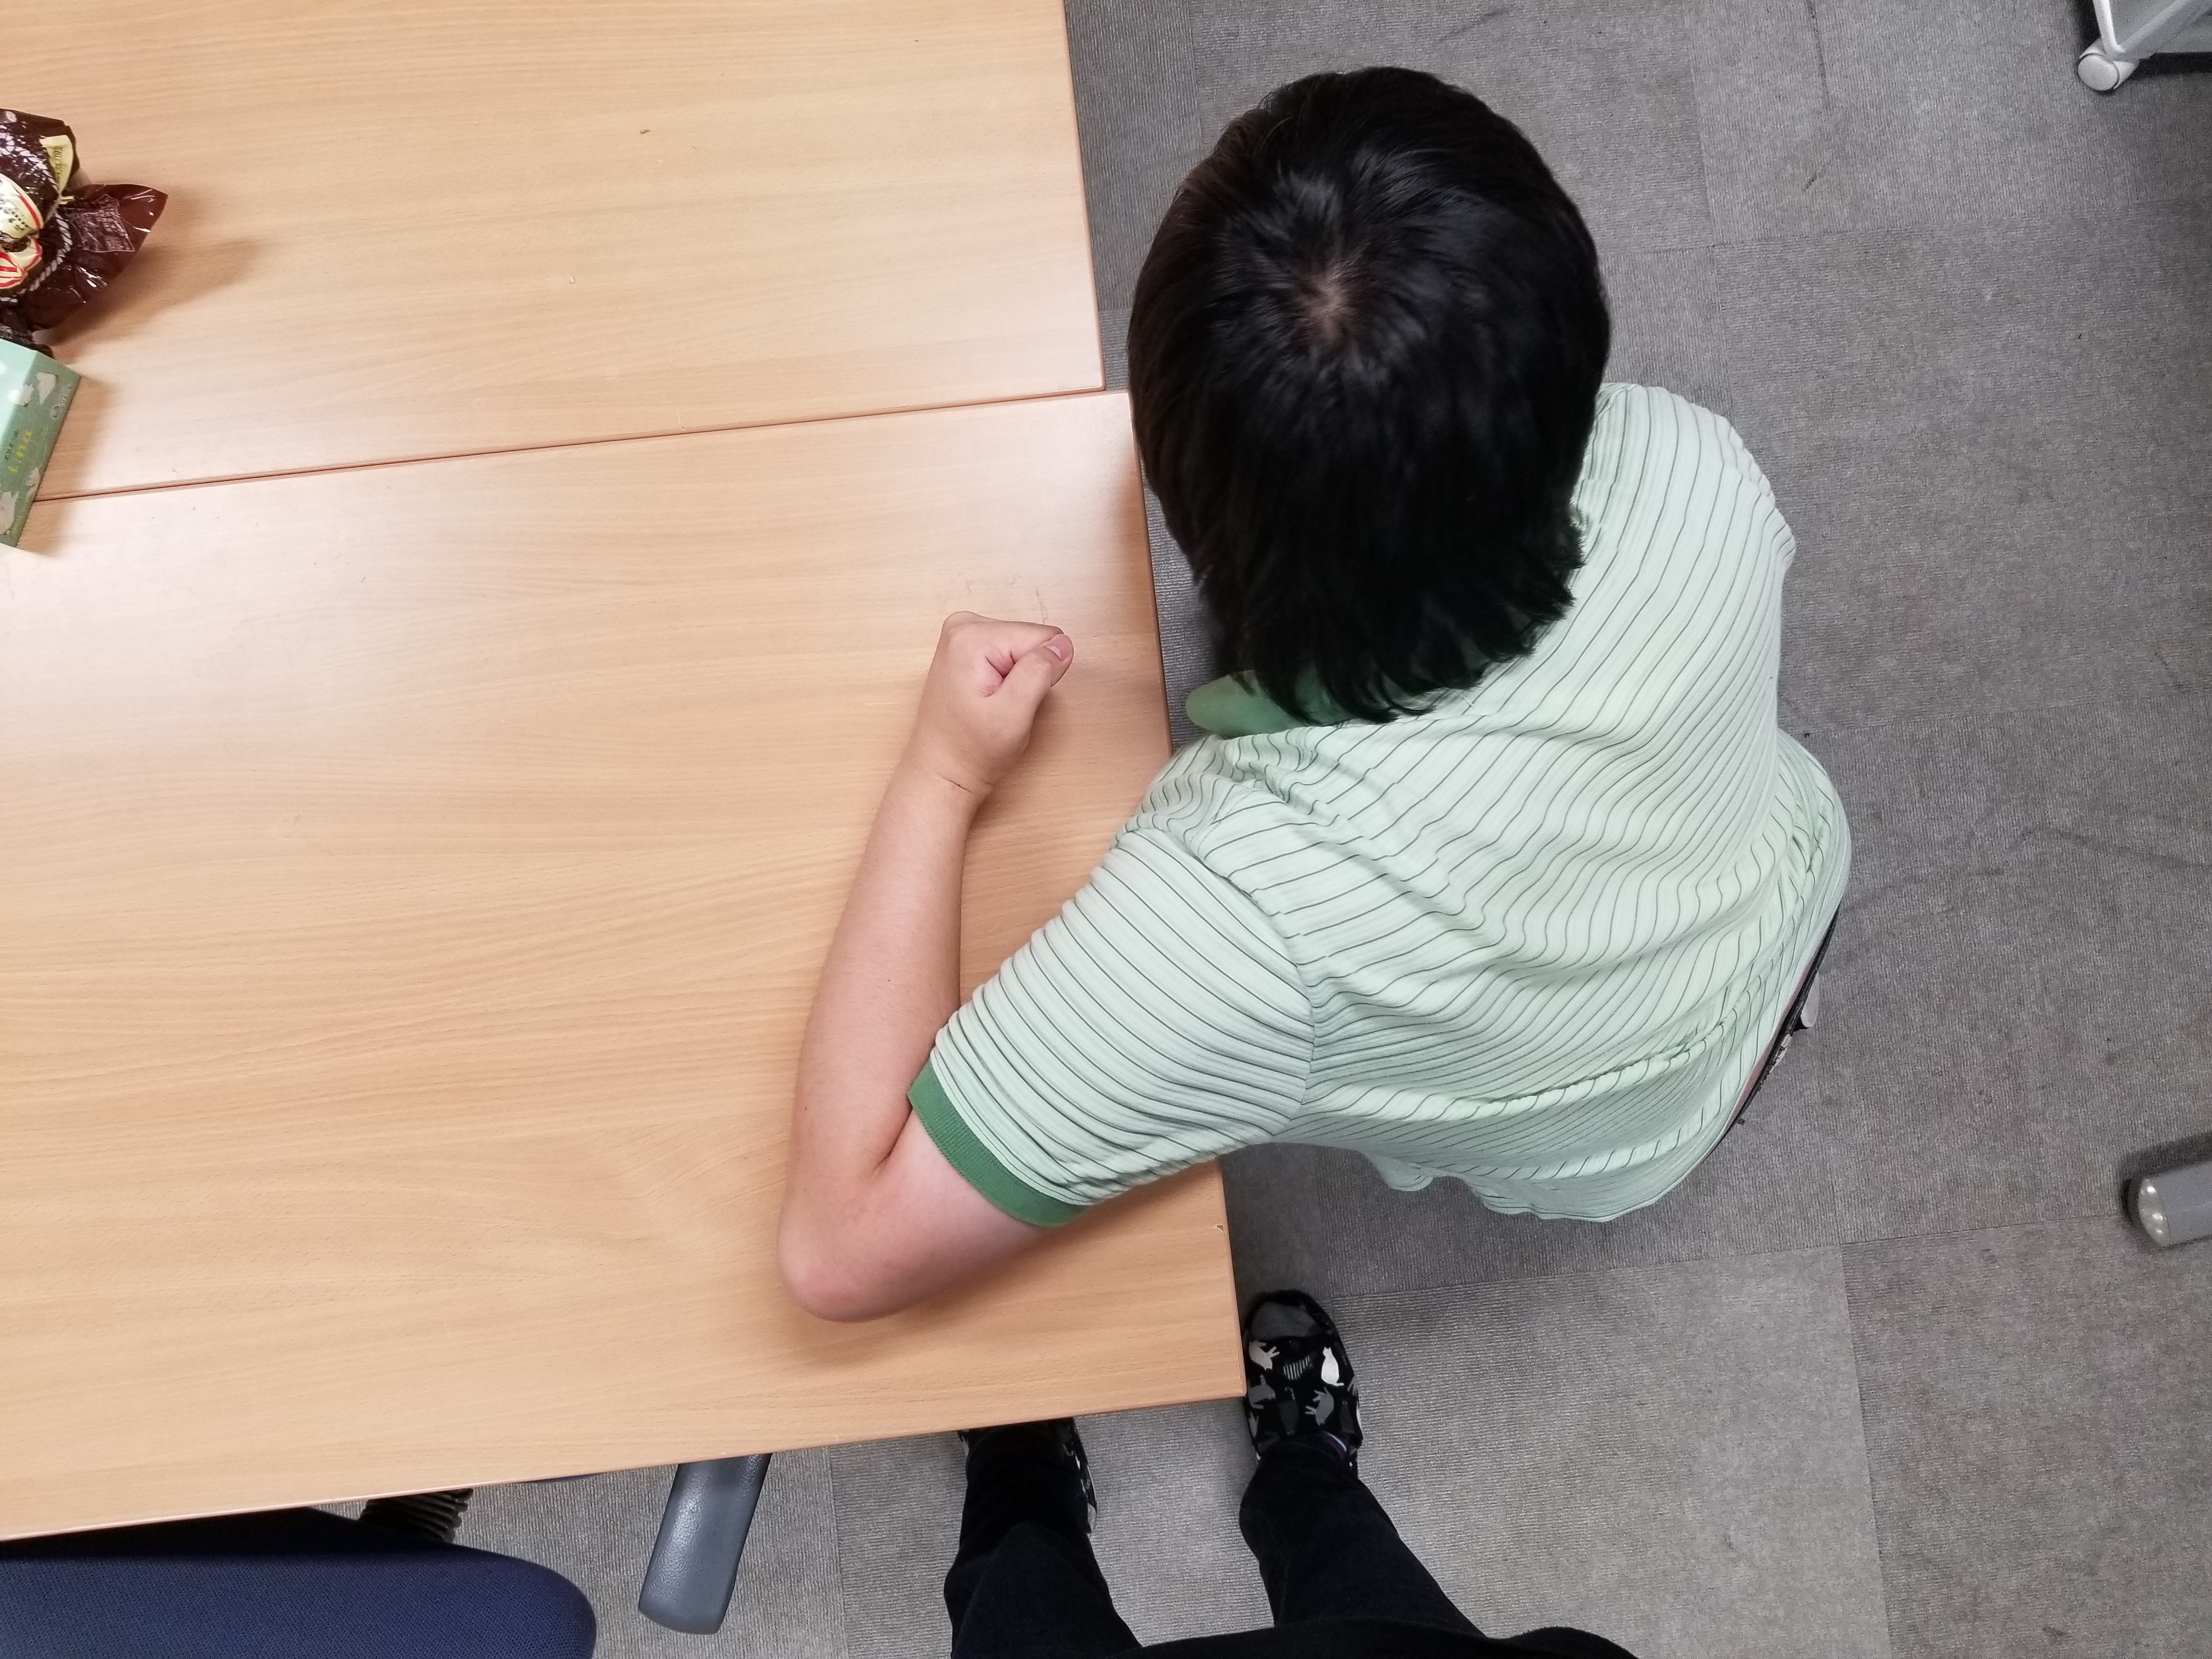
\includegraphics[width=7cm]{images/short.jpg}
    \end{center}
    \caption{腕を縮めた状態}
    \label{fig:short}
  \end{minipage}
  \begin{minipage}{0.5\hsize}
    \begin{center}
      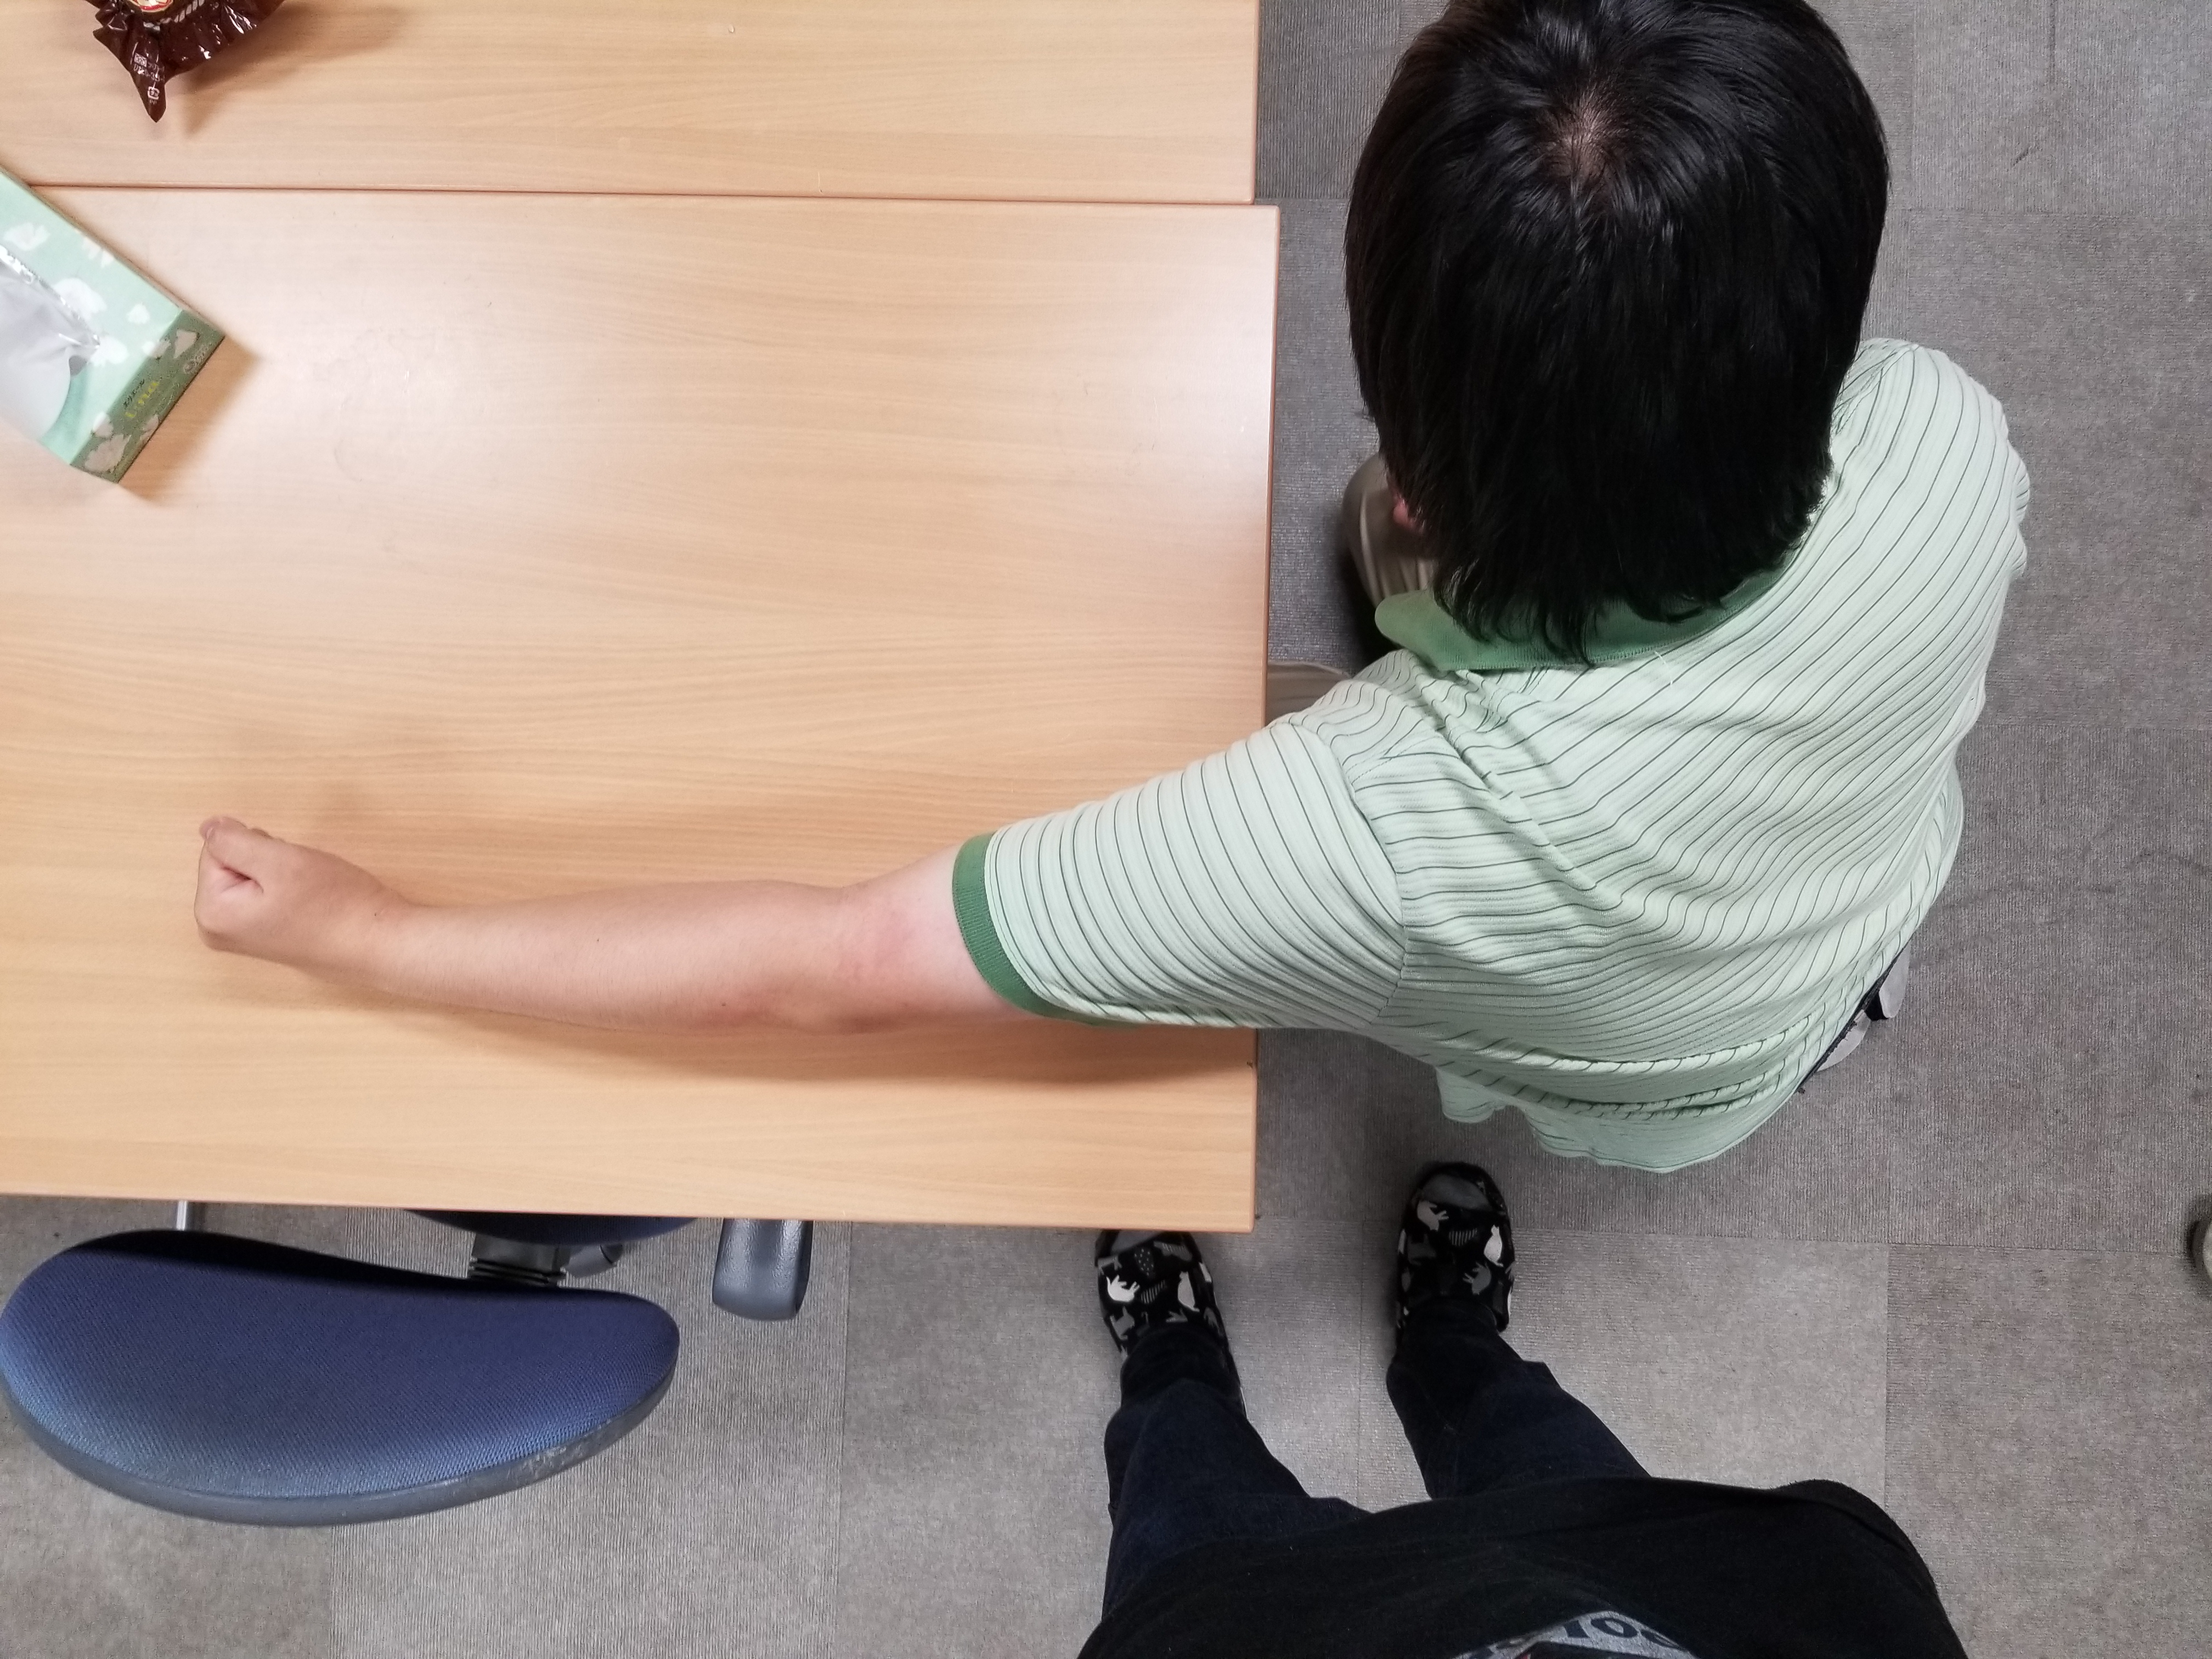
\includegraphics[width=7cm]{images/long.jpg}
    \end{center}
    \caption{腕を伸ばした状態}
    \label{fig:long}
  \end{minipage}
\end{figure}

\subsection{解析}
\subsubsection{筋電位}
筋電位のデータにはいくつかの処理を順番に施して、筋肉の活動度を求めた。
  まずデータから筋電位の特徴を抽出するために、通過帯域を1〜40 Hzとしたバンドパスフィルタ(3次バターワースフィルタ)をかけた。しかし、バンドパスフィルタをかけることによってデータに位相ズレが生じるため、時間軸を反転してもう一度同じフィルタをかけることによってこれを補正した。そしてフィルタ後のデータを整流し、時刻$t$の筋電位$|E(t)|$に対して時間$\Delta T$の間で平均を求め、筋肉の活動度とした。式は以下を用いた。
  \begin{equation}
    a(t) = \frac{1}{\Delta T} \int_{t-\frac{\Delta T}{2}}^{t+\frac{\Delta T}{2}} |E(t)| dt
  \end{equation}

\section{結果}
\begin{figure}[b]
  \begin{center}
    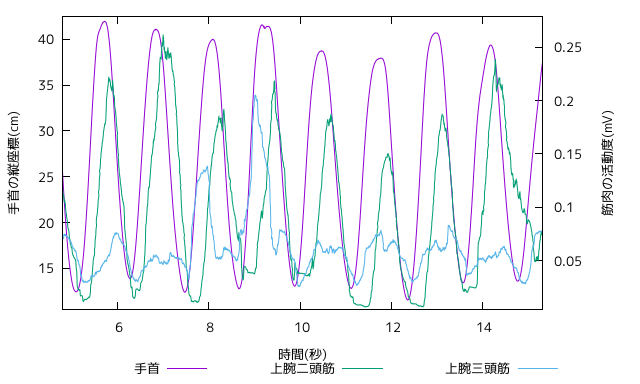
\includegraphics[width=15cm]{images/s1proto.png}
  \end{center}
  \caption{速度に関する指示のない運動と筋肉の活動度の関係}
  \label{fig:slow}
\end{figure}
図\ref{fig:slow}は、速度に関して指示を出さず腕を動かしてもらった場合である。縦軸は身体に対する手首の前後方向の変位と筋肉の活動度、横軸は時間である。手首の前後方向の変位は値が大きくなるほど体の前に伸ばしていることを示す。図中の紫、緑、青の線はそれぞれ身体に対する手首の前後方向の変位、上腕二頭筋肉の活動度、上腕三頭筋の活動度である。手首の前後方向の変位が、横方向や縦方向に比べて変位が大きく、動きが把握しやすかったからである。このグラフでは、運動開始後時刻5〜15秒の間を表示している。

例えば時刻10秒の時は、腕が屈曲した状態である。このとき腕が伸展を始め、少ししてからまず上腕三頭筋の活動度が大きくなっていっている。これは腕を伸展させるための筋活動だろう。次に、この少し後に上腕二頭筋が活動度が大きくなっていっている。これは腕がもっとも伸展した状態の前から大きくなっており、伸展の勢いを殺すために逆方向の力を加える必要があるためだろう。伸展し終わり、屈曲が始まってしばらく経つと上腕二頭筋が活動度を下げ始める。そして屈曲しきるすこし前に上腕三頭筋もその活動度を下げ始める。これは、上腕三頭筋より発達しているために、上腕二頭筋が速度に関する指示を出していない運動でも活動度の差が大きく出てしまうためであろう。活動度に大きな差があれば、当然活動度が小さい方である上腕三頭筋は腕の速度が上がりすぎるのを防ぐために活動する必要があるからである。

\begin{figure}[b]
  \begin{center}
    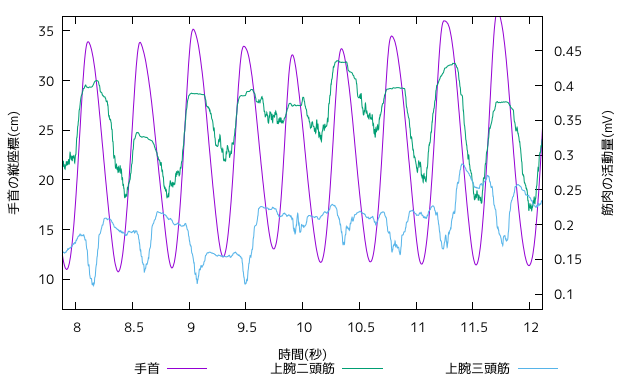
\includegraphics[width=15cm]{images/s2proto.png}
  \end{center}
  \caption{速い時の運動と筋肉の活動度の関係}
  \label{fig:fast}
\end{figure}
図\ref{fig:fast}は、腕を速く動かしてもらった場合である。各軸や凡例は図\ref{fig:slow}と同様である。このグラフでは、運動開始後時刻8〜12秒の間を表示している。図\ref{fig:fast}から、例えば時刻8.8秒の時、腕がもっとも屈曲した状態では上腕二頭筋の活動度は小さい。この状態から腕が伸展を始めると同時に活動度が大きくなっていっている。これは、上腕三頭筋による腕の伸展運動を減速、停止させるための筋活動だろう。また腕を屈曲するとともにその活動度を下げている。これは、屈曲運動をする際、もっとも筋活動が必要なのが直前の伸展運動の停止であり、それ以降は屈曲運動に速度を与えるだけなので、あまり筋活動をする必要がないからであろう。このとき上腕三頭筋は、腕をもっとも屈曲させた状態では活動度が大きく、腕が伸展させられるにしたがってその値が小さくなっていっている。これは、上腕二頭筋の逆位相のような形であり、伸展運動に速度を与えることと、屈曲運動を減速、停止させるためにしているのだろう。

図\ref{fig:slow}と図\ref{fig:fast}を比較すると、速度に関する指示を出さない場合(図\ref{fig:slow})では上腕二頭筋と上腕三頭筋の活動度はほぼ同じ位相、速く動かしてもらった場合(図\ref{fig:fast})では逆位相となっている。

\section{考察}
腕の屈伸運動をするとき、上腕二頭筋と上腕三頭筋は腕に速度を与えることの他に、二頭筋なら伸展運動、三頭筋なら屈曲運動の減速や停止のための筋活動をして身体制御を行なっているというのだろう。また、筋肉の発達度の違いから、速度によって運動時の筋活動の違いが生まれているのだろう。
\end{document}